\section{プロトタイプ検出器のデザイン}
実機と同様の構成を持つプロトタイプ検出器を製作し、性能評価試験を行うためGeant4シミュレーションによるプロトタイプ検出器の検討を行った。

\subsection{コーン型ライトガイドの深さ最適化}
今回のテスト実験では、セグメントサイズの違いによる分解能への影響を理解するために図\ref{fig:cone}の様な
2種類のコーン型ライトガイドを製作した。\\
先行研究からセグメントサイズは50 mm以下が要求されているので、入口直径は50 mmと、それより小さい30 mmのコーンを検討した。
MPPCを取り付けるため、出口直径はどちらもMPPCの対角線の長さと同じ8.5 mmとした。
各コーンの深さによって集光効率が変わるため、最適な深さをGEANT4によるシミュレーションを用いて決定した。\\\indent

図\ref{fig:cone_optimize}の様にコーン入口に対して垂直・一様に光子を入射させ、コーンの入口と出口での光子数を測定した。
コーンは厚さ$\SI{1}{mm}$のAlとし、入口は外側の直径がセグメントサイズに対応するため、外側の直径をそれぞれ$\SI{50}{mm}$と$\SI{30}{mm}$とした。
出口は内側にMPPCを取り付ける必要があるため、内側の直径をともに$\SI{8.5}{mm}$とした。
また、Alの反射率は図\ref{fig:Al_reflection}を参考に波長依存性を考慮して設定した。
コーンの収率を、
\begin{equation}
  \label{eq:cone_yield}
  \mbox{収率} = \frac{\mbox{出口での光子数}}{\mbox{入口での光子数}}
\end{equation}
とし、コーンの深さに対する収率を調べた。その結果を図\ref{fig:cone50_optimize}、\ref{fig:cone30_optimize}に示す。
\begin{figure}
  \centering
  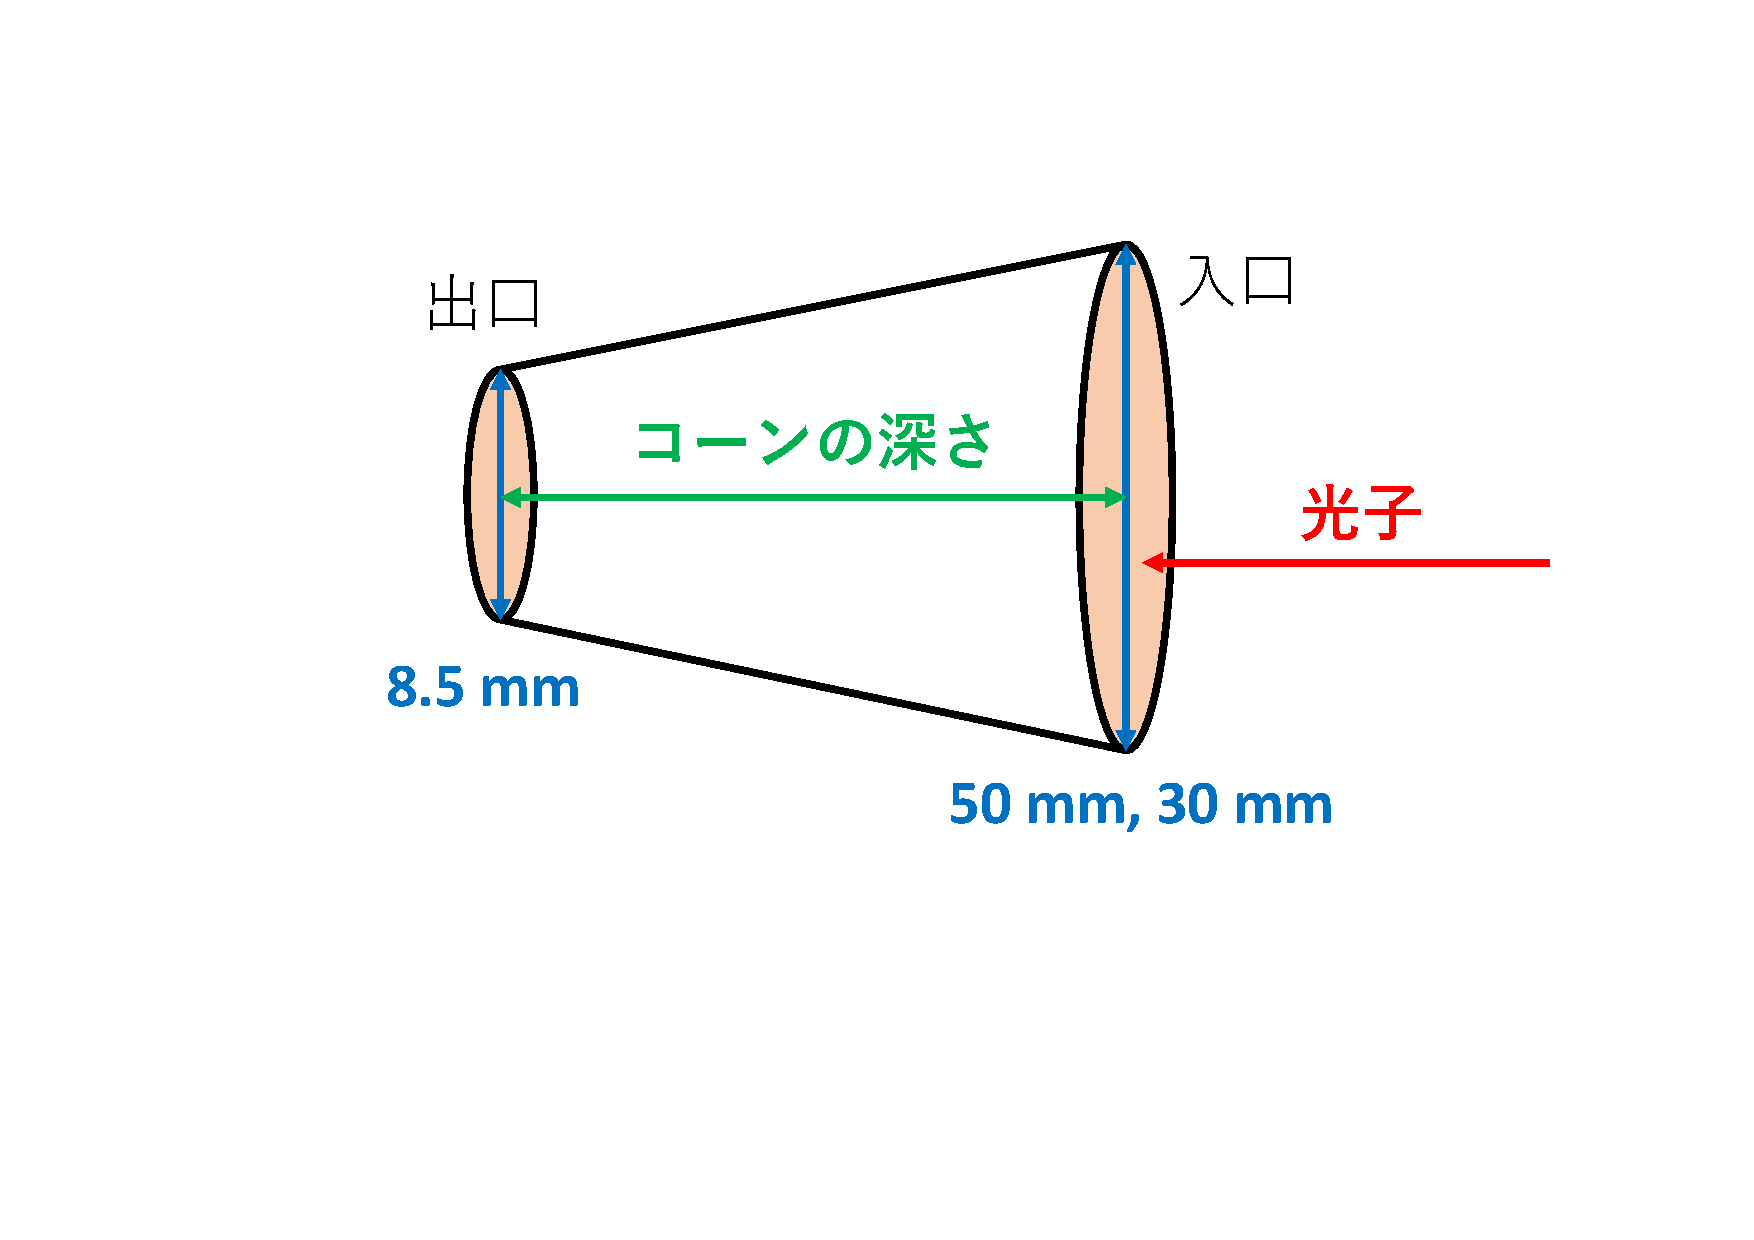
\includegraphics[width=10cm]{images/chapter3/cone_optimize.pdf}
  \caption{Geant4シミュレーションの模式図。コーンの深さを変えながら収率を確認した。}
  \label{fig:cone_optimize}
\end{figure}

\begin{figure}
  \centering
  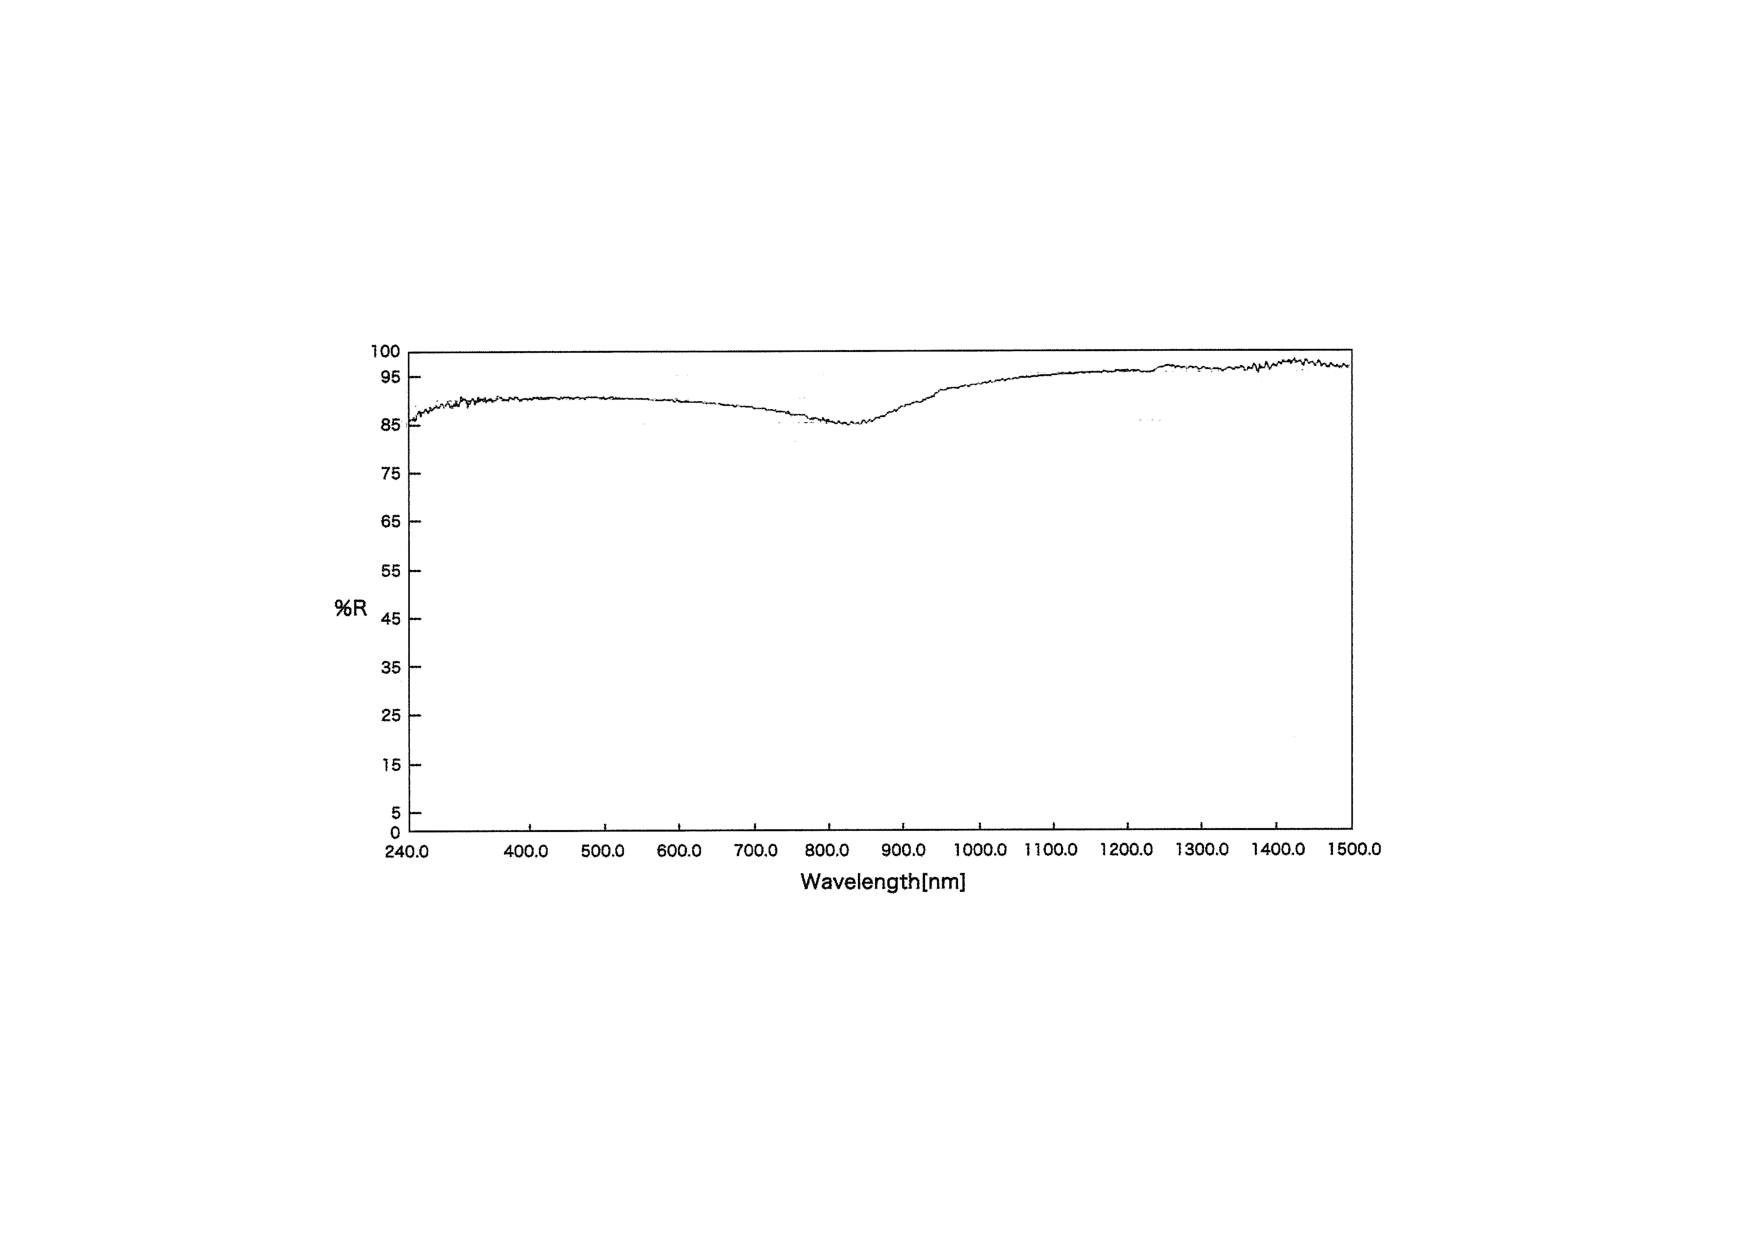
\includegraphics[width=15cm]{images/chapter3/Al_reflection.pdf}
  \caption{アルミコートの反射率の波長依存性\cite{ref7}。}
  \label{fig:Al_reflection}
\end{figure}

\begin{figure}[htbp]
  \begin{tabular}{cc}
    %---- 最初の図 ---------------------------
    \begin{minipage}[t]{0.45\hsize}
      \centering
      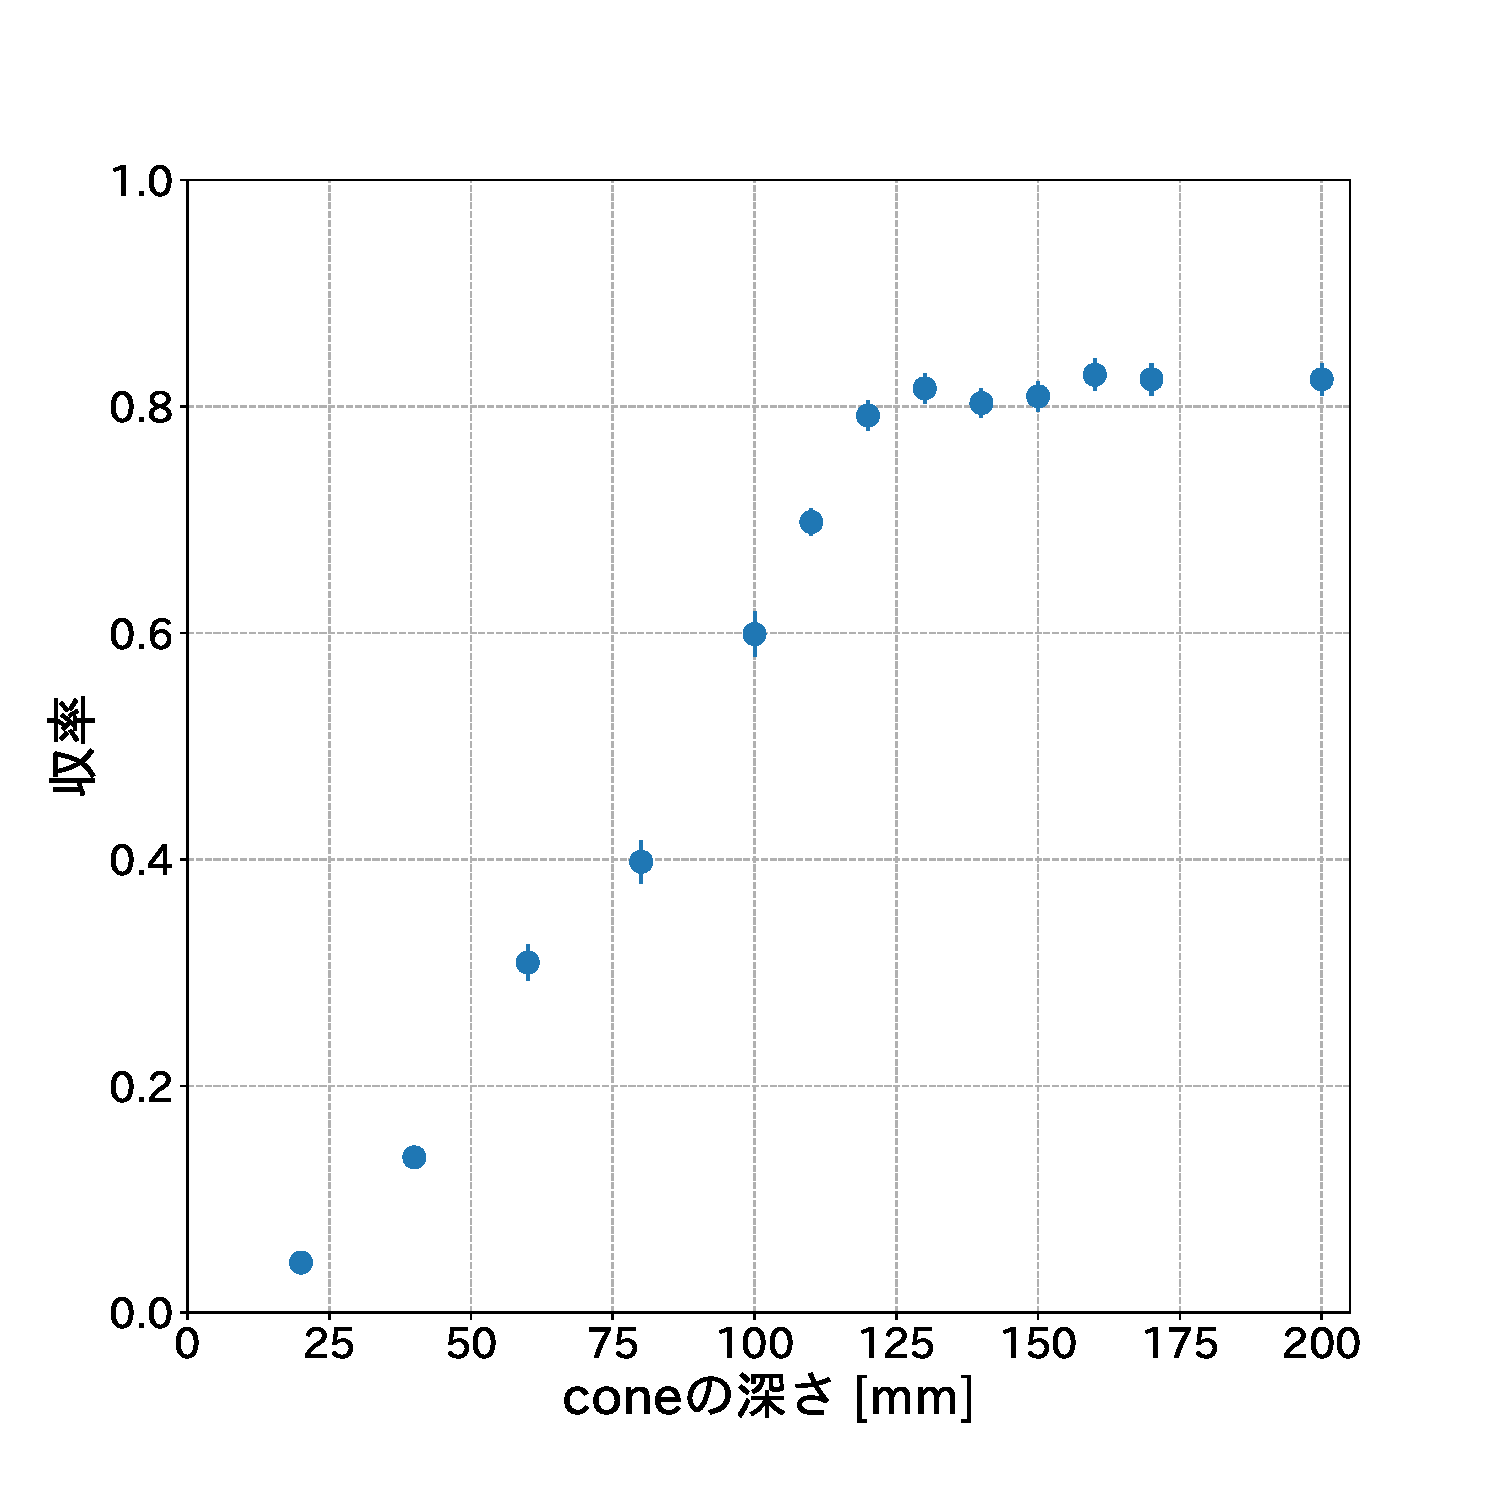
\includegraphics[keepaspectratio, scale=0.3]{images/chapter3/cone50_optimize.pdf}
      \caption{平行光が入射した場合の$\SI{50}{mm}$コーンの深さに対する収率。深さ$\SI{110}{mm}$でサチュレーションする。}
      \label{fig:cone50_optimize}
    \end{minipage} &
    %---- 2番目の図 --------------------------
    \begin{minipage}[t]{0.45\hsize}
      \centering
      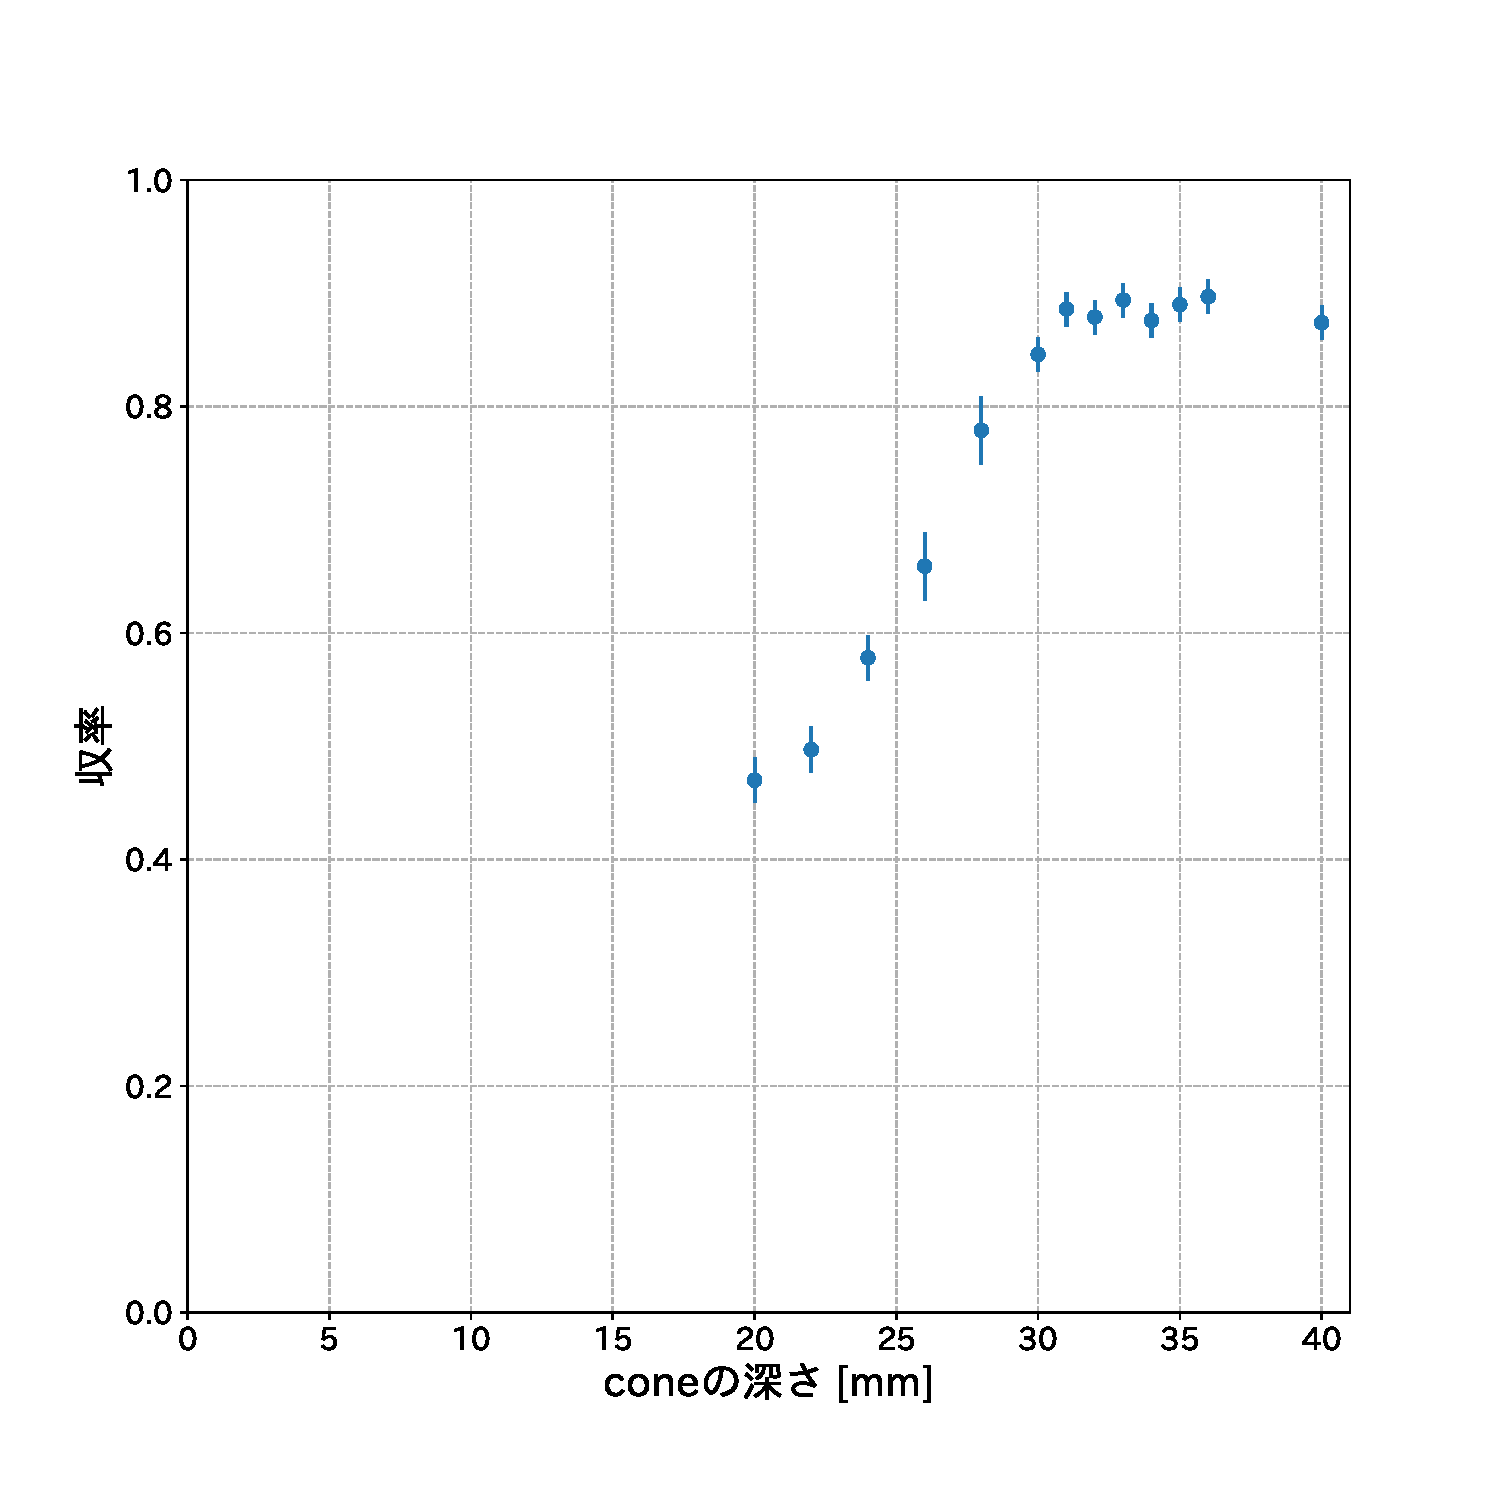
\includegraphics[keepaspectratio, scale=0.3]{images/chapter3/cone30_optimize.pdf}
      \caption{平行光が入射した場合の$\SI{30}{mm}$コーンの深さに対する収率。深さ$\SI{31}{mm}$でサチュレーションする。}
      \label{fig:cone30_optimize}
    \end{minipage}
    %---- 図はここまで ----------------------
  \end{tabular}
\end{figure}
\noindent50 mmコーンは110 mm, 30 mmコーンは31 mmで収率がサチュレーションすることが分かった。\\\indent

続いて、図\ref{fig:cone_optimize2}光子が検出面に対して角度を持って一様に入射した場合の収率について、サチュレーションした付近のコーンの深さで調べた。
$\SI{50}{mm}$コーンは深さ$\SI{110}{mm}$、$\SI{120}{mm}$、$\SI{130}{mm}$、
$\SI{30}{mm}$コーンは深さ$\SI{31}{mm}$、$\SI{32}{mm}$、$\SI{33}{mm}$で比較を行なった。
その結果を図\ref{fig:cone50_optimize2}, \ref{fig:cone30_optimize2}に示す。
コーンの深さを深くすると、角度のついた入射粒子に対して収率が良くなることがわかった。
また、工作精度の影響を抑えるために、コーンの深さは図\ref{fig:cone50_optimize}, \ref{fig:cone30_optimize}でサチュレーションし出した深さよりも少し深めの
$\SI{50}{mm}$コーンは深さ$\SI{120}{mm}$、$\SI{50}{mm}$コーンは深さ$\SI{33}{mm}$を採用した。

\begin{figure}
  \centering
  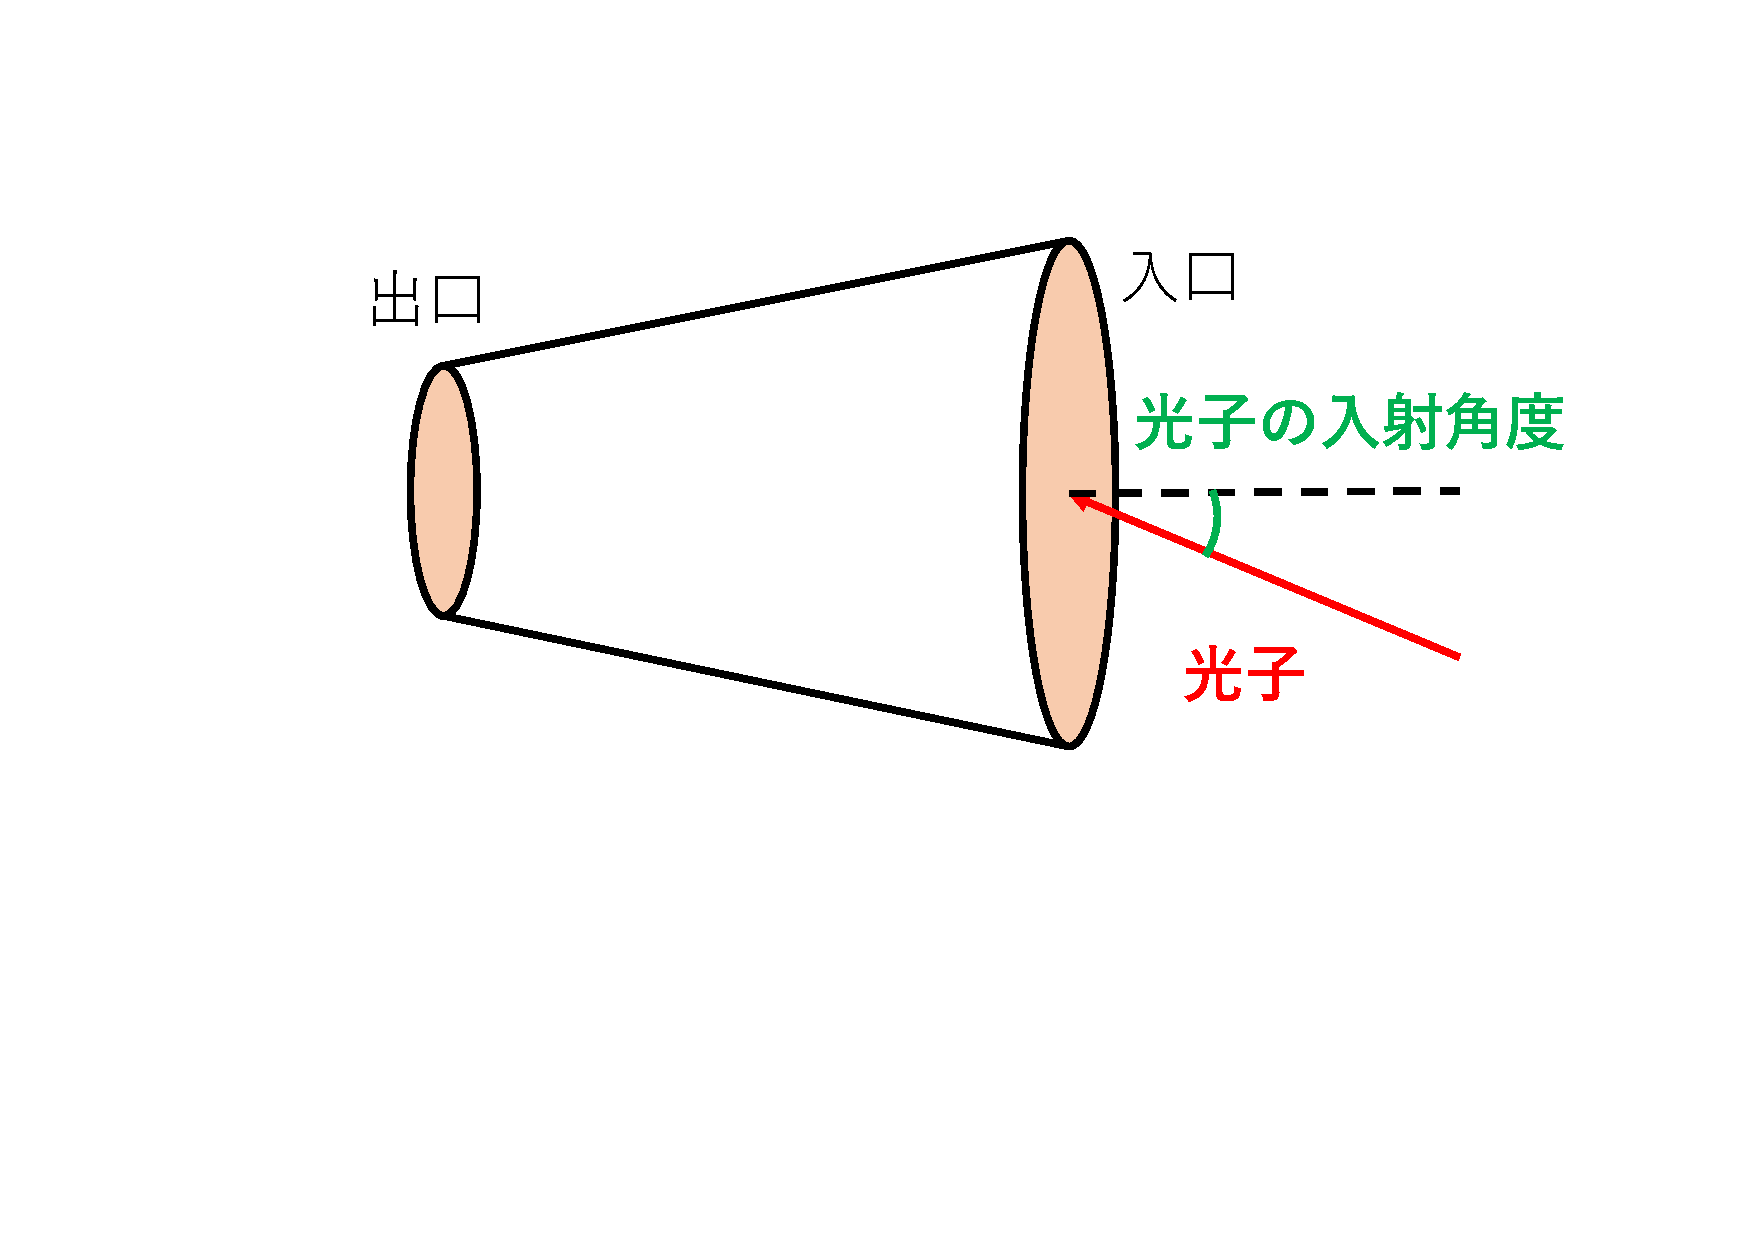
\includegraphics[width=10cm]{images/chapter3/cone_optimize2.pdf}
  \caption{Geant4シミュレーションの模式図。光子の入射角度を変えながら収率を確認した。}
  \label{fig:cone_optimize2}
\end{figure}

\begin{figure}[htbp]
  \begin{tabular}{cc}
    %---- 最初の図 ---------------------------
    \begin{minipage}[t]{0.45\hsize}
      \centering
      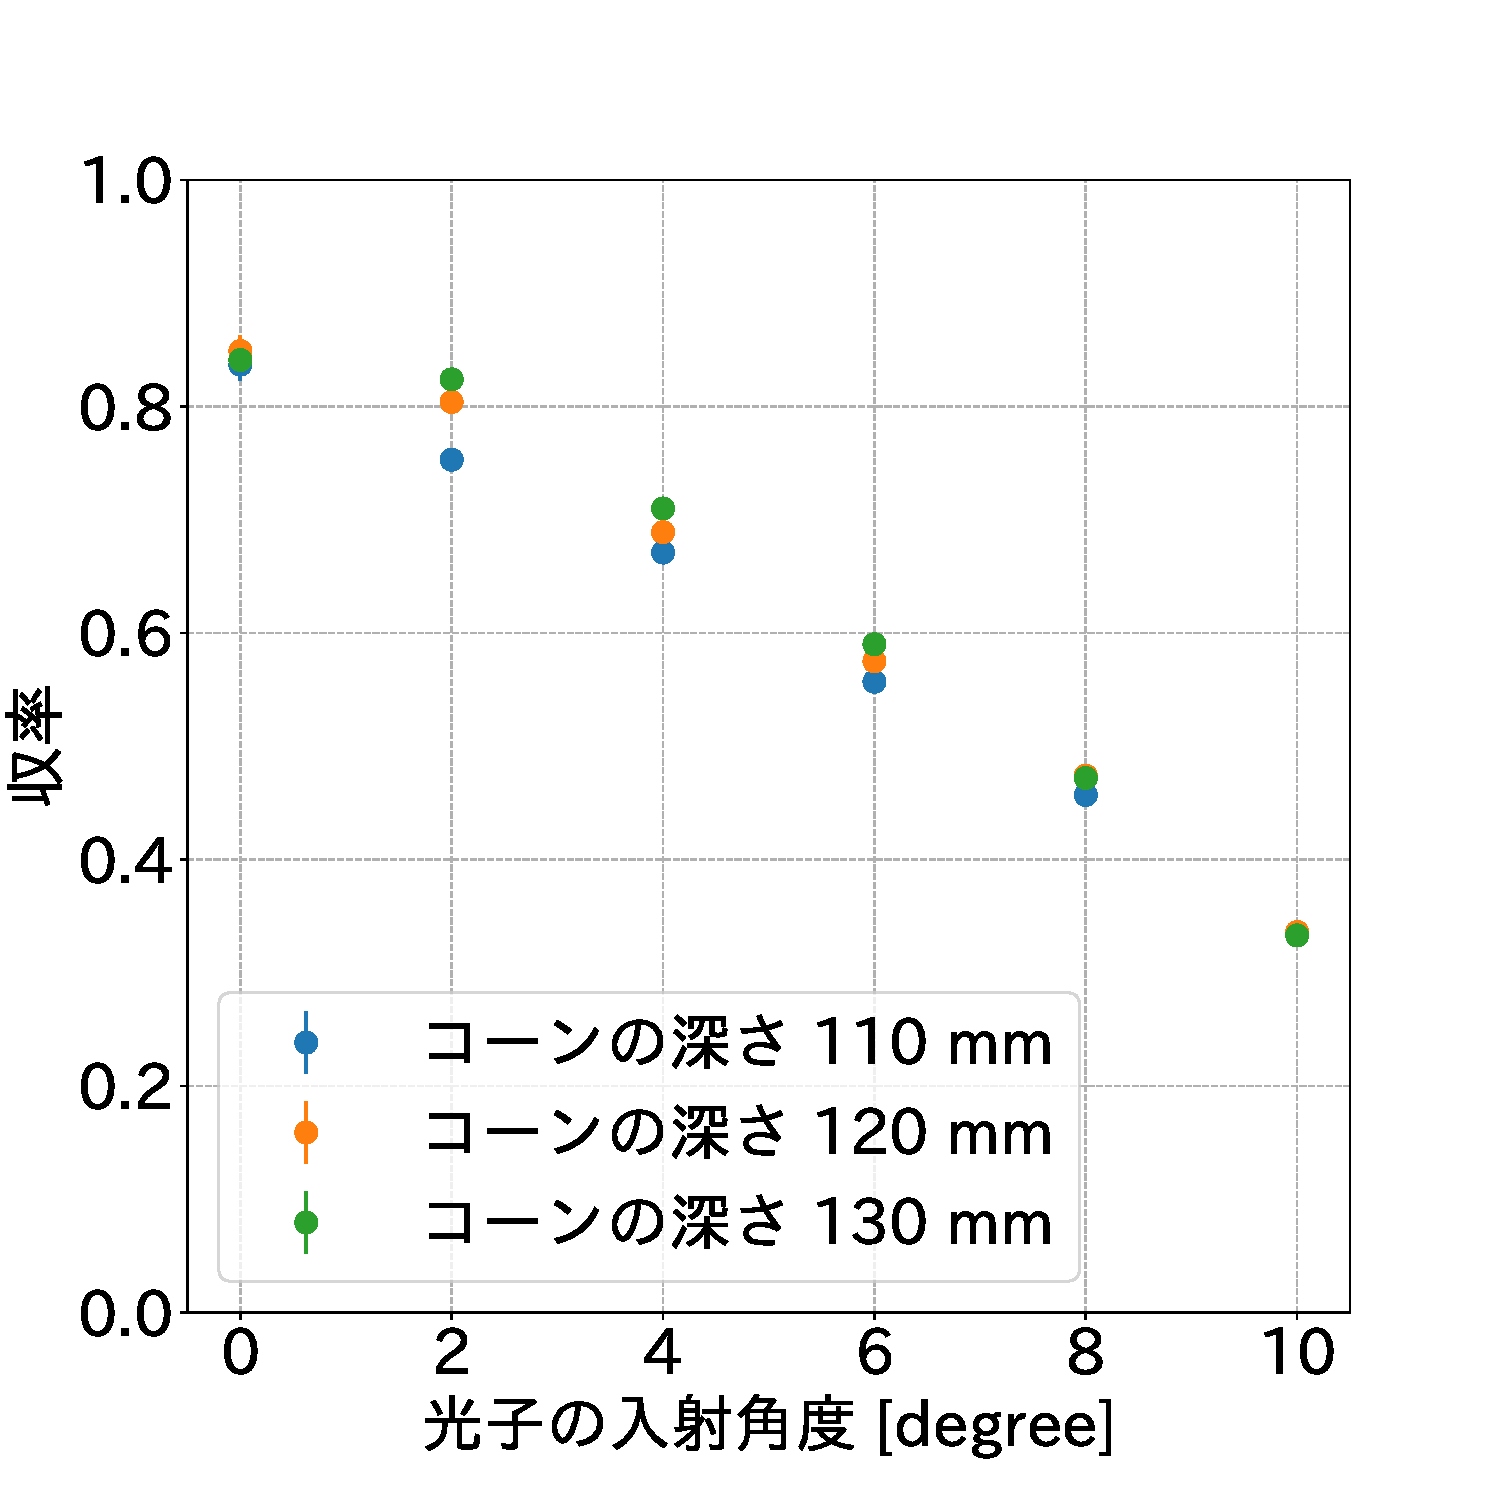
\includegraphics[keepaspectratio, scale=0.3]{images/chapter3/cone50_optimize2.pdf}
      \caption{$\SI{50}{mm}$コーンの光子の入射角度に対する収率。}
      \label{fig:cone50_optimize2}
    \end{minipage} &
    %---- 2番目の図 --------------------------
    \begin{minipage}[t]{0.45\hsize}
      \centering
      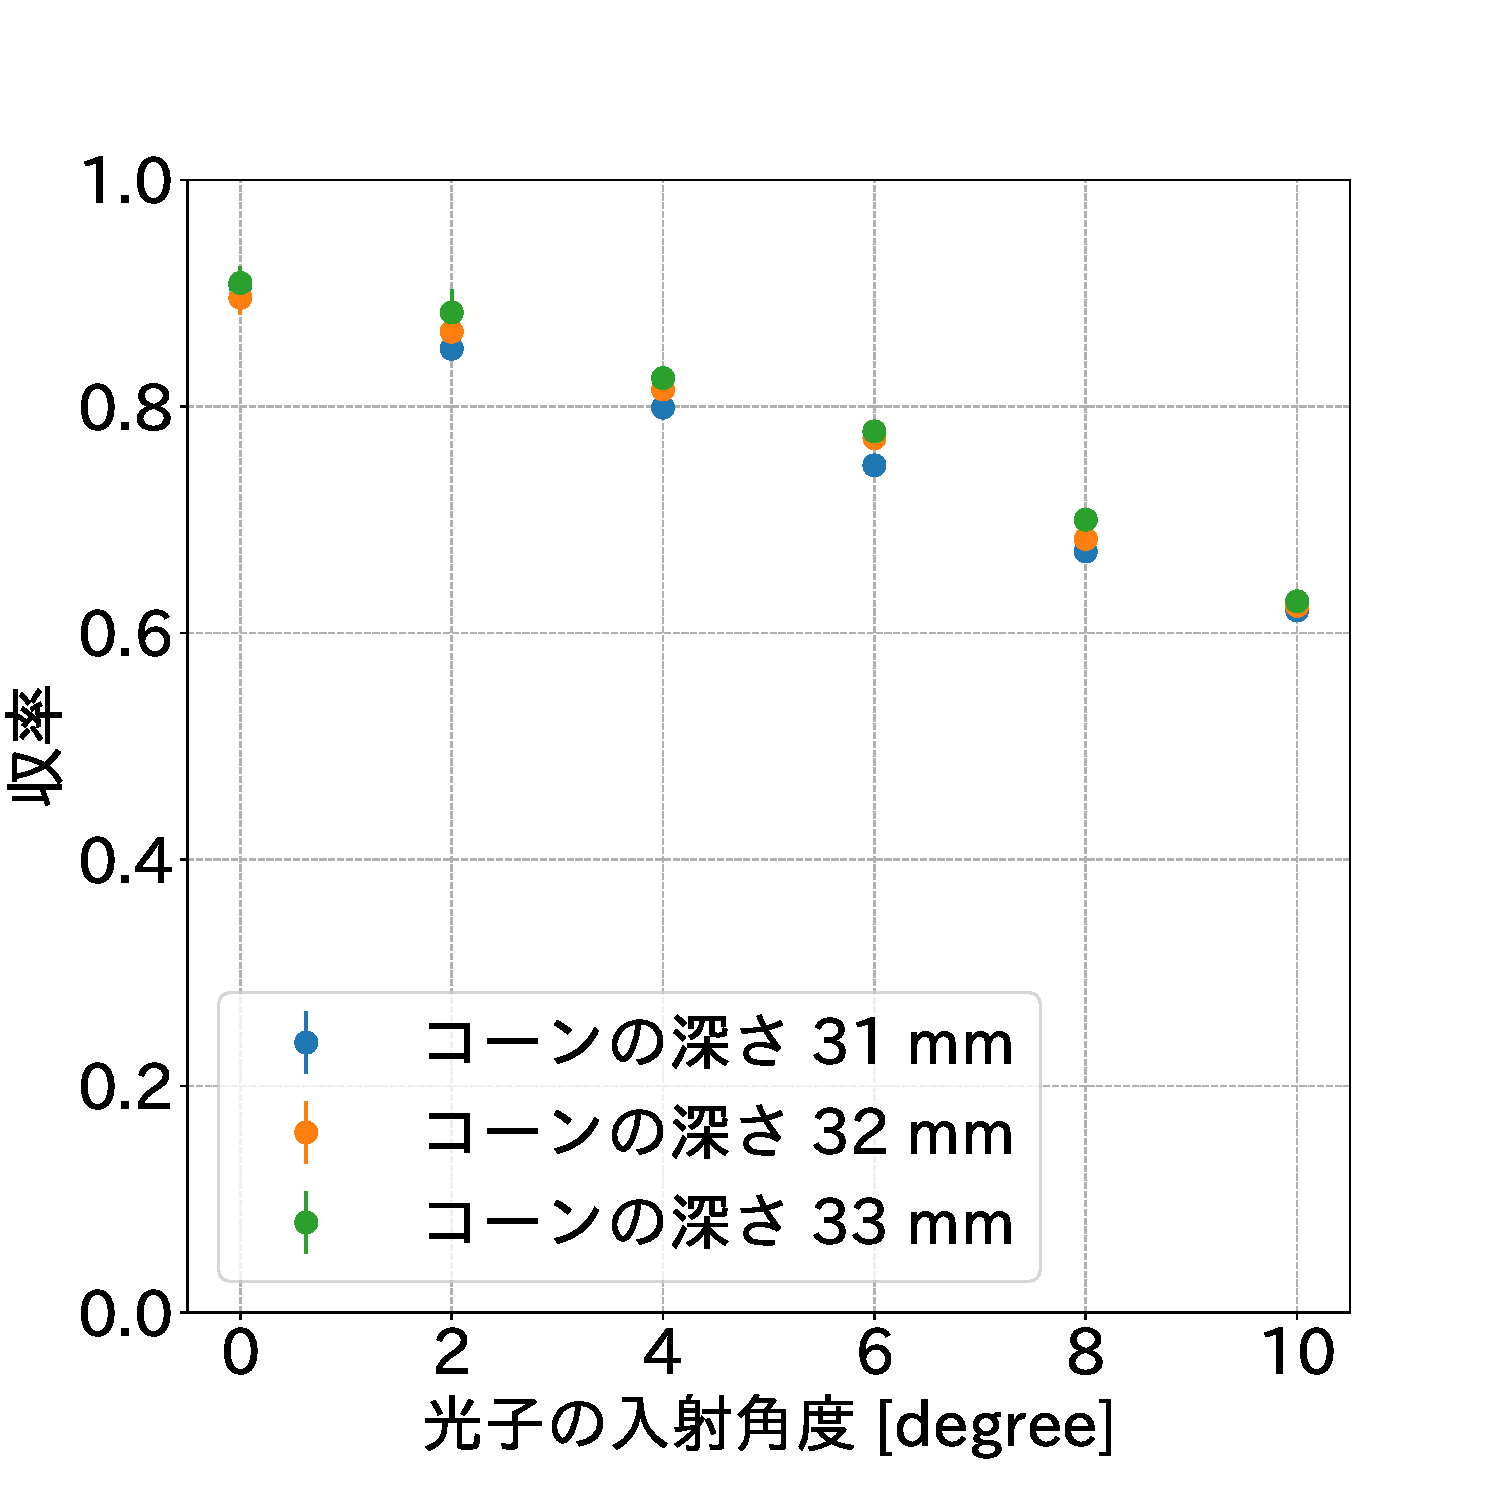
\includegraphics[keepaspectratio, scale=0.3]{images/chapter3/cone30_optimize2.pdf}
      \caption{$\SI{30}{mm}$コーンの光子の入射角度に対する収率。}
      \label{fig:cone30_optimize2}
    \end{minipage}
    %---- 図はここまで ----------------------
  \end{tabular}
\end{figure}